%
% File NLP4MusA.tex
%
%% Based on the style files for NLP4MusA 2020, which were
%% Based on the style files for ACL 2018, NAACL 2018/19, which were
%% Based on the style files for ACL-2015, with some improvements
%%  taken from the NAACL-2016 style
%% Based on the style files for ACL-2014, which were, in turn,
%% based on ACL-2013, ACL-2012, ACL-2011, ACL-2010, ACL-IJCNLP-2009,
%% EACL-2009, IJCNLP-2008...
%% Based on the style files for EACL 2006 by 
%%e.agirre@ehu.es or Sergi.Balari@uab.es
%% and that of ACL 08 by Joakim Nivre and Noah Smith

\documentclass[11pt,a4paper]{article}
\usepackage[hyperref]{nlp4MusA}
\usepackage{times}
\usepackage{latexsym}
\usepackage{graphicx}
\usepackage{mathtools}  % amsmath with extensions
\usepackage{amsfonts}  % (otherwise \mathbb does nothing)
\usepackage{url}


%\aclfinalcopy % Uncomment this line for the final submission
%\def\aclpaperid{100} %  Enter the acl Paper ID here

%\setlength\titlebox{5cm}
% You can expand the titlebox if you need extra space
% to show all the authors. Please do not make the titlebox
% smaller than 5cm (the original size); we will check this
% in the camera-ready version and ask you to change it back.

\newcommand\BibTeX{B\textsc{ib}\TeX}


\title{Shift-Invariant Dictionary Learning using TCN-WTA Autoencoders for Discovering Musical Relations }

\author{First Author \\
  Affiliation / Address line 1 \\
  Affiliation / Address line 2 \\
  Affiliation / Address line 3 \\
  \texttt{email@domain} \\\And
  Second Author \\
  Affiliation / Address line 1 \\
  Affiliation / Address line 2 \\
  Affiliation / Address line 3 \\
  \texttt{email@domain} \\}

\date{}

\begin{document}
\maketitle
\begin{abstract}
Music temporal structure is full of shift-invariant patterns (e.g. motifs, ostinatos, loops, samples, etc.).  We propose using a using a Fully Convolutional Temporal Autoencoder (FCTA) with a k-Winner Takes All (k-WTA) activation function to find a shift-invariant dictionary to represent symbolic, multivariate, musical signals. We train our model to represent fixed drum tracks and variable length piano music. We show few applications of this sparse representation such as de-noising musical ideas, unsupervised stylistic segmentation, and music generation. To assist related work, we have made interactive code available along with the trained models 



\end{abstract}

\section{Introduction}

The dictionary learning framework, aims at finding a sparse representation of the input data (sparse coding) in the form of a linear combination of basic elements we call atoms. There are multiple benefits in obtaining a sparse encoding of a signal. To name a few, they are lightweight— requiring less memory to store and allowing faster inference and easier interpretability and they can encode prior knowledge in the sparsity patterns. In addition, sparsity provides a way to discern patterns in an informed and principled manner . 

 Sparse dictionary learning has led to state-of-art results in various image and video processing tasks as well as to texture synthesis \cite{Peyre2009} and unsupervised clustering \cite{Ramrez2010ClassificationAC} . In evaluations with the Bag-of-Words model \cite{7439823}, sparse coding was found empirically to outperform other coding approaches on the object category recognition tasks.  
 
The ability to dis til complex data structures such as music down to sets of dictionaries—salient features of a specific performer or music, has a multitude of applictions in music.  Music transcription and classification tasks have seen a strong usage of sparse dictionary learning in the past \cite{Grosse2007} \cite{Costantini2013}, \cite{Blumensath2006}, \cite{SrinivasM2014}, \cite{Srinivas2014}, \cite{Cogliati2016}. Nonetheless, we have yet to see a study that harnesses the advantages of sparse representation for the purpose of music creation. Instead, the popular methods for discovering music relations and achieving music generation have been a transformer with some sort of attention mechanism or the recurrent architectures. \cite{JiangJunyan2020} for instance, uses an attention module that is tailored to the discovery of sequence level relations in music, while studies like \cite{Roberts2018} uses the recurrent variational autoencoder and a hierarchical decoder in order to model long-term musical structures. In our study we explore applications of sparse representation such as de-noising musical ideas, unsupervised stylistic segmentation, and music generation.
 

% ConvNets were subsequently
%applied to NLP tasks such as part-of-speech tagging and
%semantic role labelling (Collobert ; Weston, 2008; Collobert et al., 2011; dos Santos ; Zadrozny, 2014). More
%recently, convolutional networks were applied to sentence
%classification (Kalchbrenner et al., 2014; Kim, 2014) and
%document classification (Zhang et al., 2015; Conneau et al.,
%2017; Johnson ; Zhang, 2015; 2017). Particularly inspiring
%for our work are the recent applications of convolutional
%architectures to machine translation (Kalchbrenner et al.,
%2016; Gehring et al., 2017a;b), audio synthesis (van den
%Oord et al., 2016), and language modeling (Dauphin et al.,
%2017).


\section{Related Work}


\subsection{ Dictionary learning  }
Given the data: $ X=\left[x_{1}, \ldots, x_{K}\right], x_{i} \in \mathbb{R}^{d} $ 
We want a dictionary $\mathbf{D} \in \mathbb{R}^{d \times n}: D=\left[d_{1}, \ldots, d_{n}\right]$ 
And a representation $R=\left[r_{1}, \ldots, r_{K}\right], r_{i} \in \mathbb{R}^{n}$ such that the reconstruction $\|X-\mathbf{D} R\|_{F}^{2}$ is minimized and $r_{i}$ are sparsed. The optimization problem can be formulated as: 

$\underset{\mathbf{D} \in \mathcal{C}, r_{i} \in \mathbb{R}^{n}, \lambda>0} {\operatorname{argmin}} \sum_{i=1}^{K}\left\|x_{i}-\mathbf{D} r_{i}\right\|_{2}^{2}+\lambda\left\|r_{i}\right\|_{0}$ \\   $\mathcal{C} \equiv\left\{\mathbf{D} \in \mathbb{R}^{d \times n}:\left\|d_{i}\right\|_{2} \leq 1 \forall i=1, \ldots, n\right\} $
\\ \\
There are various methods to solve this problem, however this formulation does not look for shift invariant features. The dictionary components are the same size as original signal we are seeking to recustruct.

\subsection{ Shift-invariant dictionary learning (SIDL)  }

Shift-invariant dictionary learning (SIDL) refers to the problem of discovering a latent basis that captures local patterns at different locations of input signal, and a sparse coding for each sequence as a linear combination of these elements \cite{Zheng2016} 

This has a similar formulation as eq.1 except to reconstruct we have to stride along our signal. We can rewrite \\
$\mathbf{D} r_{i} \longrightarrow \sum_{k=1}^{K} \boldsymbol{r}_{i k} T\left(\mathbf{d}_{k}, t_{i k}\right)$
\\
where \\
$T_{p}(\mathbf{d}, t) \ =\begin{cases}\mathbf{d}_{i-t} & \text { if } 1 \leq i-t \leq q \\ 0 & \text { otherwise }\end{cases}$

here $t_{i k}$ corresponds first location where $d_k$ matches our signal. Therefore, $t_{i k}=0$ indicating that $\mathbf{d}_{k}$ is aligned to the beginning of $\mathbf{x}_{i}$ and that $t_{i k}=p-q$ indicating the largest shift $\mathbf{d}_{k}$ can be aligned to $\mathbf{x}_{i}$ without running beyond


In previous works, various shift-invariant dictionary learning (SIDL) methods have been employed to discover local patterns that are embedded across a longer time series in sequential data such as audio signals. While \cite{Grosse2007} employs shift-
invariant sparse coding with a convolutional optimization and gradient descent method for an audio classification task, \cite{Zheng2016} demonstrates an efficient algorithm with the ability to combine shift-invariant patterns in a sparse coding of the original data for audio reconstruction and classification tasks. 
%Such unsupervised learning methods have shown to be powerful in discovering shift-invariant patterns and a handful of studies have implemented SIDL for the purpose of music. 



\subsection{Temporal Convolutional Networks (TCN) }

Recent results suggest that TCNs convincingly outperform
baseline recurrent architectures across a broad range of sequence modeling tasks.

The distinguishing characteristics of TCNs are: 1)
the convolutions in the architecture are causal, meaning that
there is no information “leakage” from future to past; 2) the
architecture can take a sequence of any length and map it to
an output sequence of the same length, just as with an RNN.

To put it simply: TCN = 1D FCN + causal convolutions.

This architecture is informed by recent convolutional architectures for sequential data \cite{oord2016wavenet},
\cite{kalchbrenner2017neural} ; \cite{DBLP:journals/corr/DauphinFAG16}; \cite{Zheng2016}, TCN have several advantages, for example,
the TCN is much simpler than WaveNet (van den Oord et al.,
2016) (no skip connections across layers, conditioning, context stacking, or gated activations).
Compared to the language modeling architecture of Dauphin
et al. (2017), TCNs do not use gating mechanisms and have
much longer memory. 



\subsection{SIDL by TCN K-WTA Autoencoders}
To learn the shift invariant dictionaries, we use a convolutional k-winner-take-all autoencoder \cite{DBLP:journals/corr/MakhzaniF14}. This is a standard convolutional autoencoder except after training the encoder, the single largest hidden activity of each feature map is kept and the rest (as well as their derivatives) are set to zero. Next, the decoder reconstructs the output from the sparse feature maps. This results in a sparse representation where the sparsity level is the number of non-zero feature maps. \emph{If a shallow decoder (1 layer) is used, the kernel weights of the decoder are the atoms of the dictionary used to reconstruct the signal}. 

In theory, all we need to learn a dictionary is a Ecoder-Decoder 1D-Conv layers to generate a sprase representation. However, if our signal is dense, learning can improve if we add a TCN Layer to extract temporal features. This TNC can have variable depth depending on the task.

\begin{figure}[ht]
  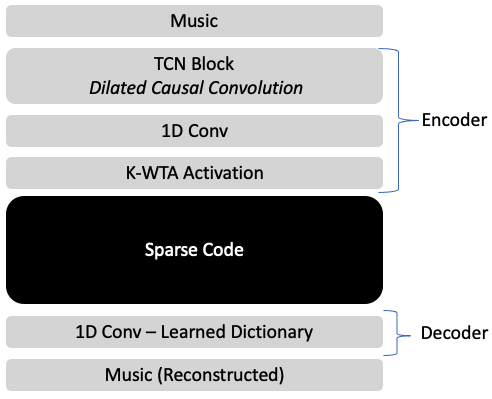
\includegraphics[width=\linewidth]{/Users/juanhuerta/personal_projects/code/shift_invariant_dictionary_learning/paper/images/tcn.png}
  \caption{After training the model we can use it to encode datapoints of arbitrary length unsupervised stylistic segmentation. We use PCA on the average sparse code for each piece. We project into 2 dimensional sparse to visualize }
  \label{fig:boat1}
\end{figure}

\begin{figure*}[ht]
  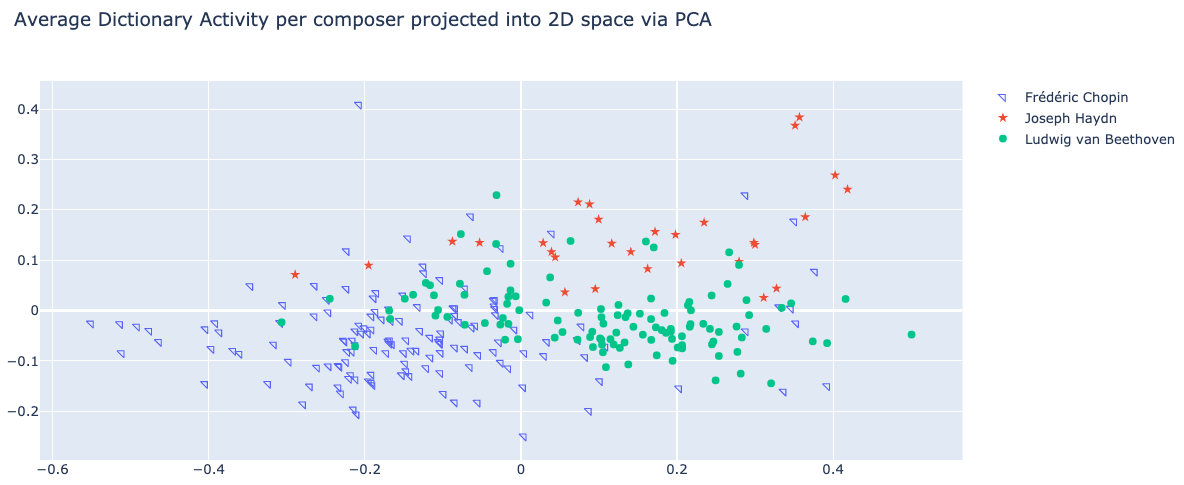
\includegraphics[width=\linewidth]{/Users/juanhuerta/personal_projects/code/shift_invariant_dictionary_learning/paper/images/newplot.png}
  \caption{After training the model we can use it to encode datapoints of arbitrary length unsupervised stylistic segmentation. We use PCA on the average sparse code for each piece. We project into 2 dimensional sparse to visualize }
  \label{fig:boat1}
\end{figure*}




\section{Experiments}
\label{ssec:experiments}

We show a few applications of our TCN k-WTA model, De-noising musical ideas; Unsupervised stylistic segmentation; Music generation. We do this for two distinct datasets with different MIDI encodings.


\subsection{Datasets}
\label{ssec:experiments}

We use two distinct datasets: MAESTRO  \cite{hawthorne2018enabling}, and  grove Groove  \cite{groove2019} . See table 2 for more details on the datasets used. We also use distinct MIDI representations for each dataset. 

\begin{table*}[ht]
    \centering
    \begin{tabular}{p{0.15\linewidth} | p{0.15\linewidth} | p{0.1\linewidth}  | p{0.45\linewidth} }
      Dataset  & Size  & Instrument &  MIDI Representation\\ \hline
      Maestro  & 1020 (Hrs)   & Piano &  One-hot encoding over 388 different MIDI events. Every datapoint here has an arbitrary length \\
        \hline
        Groove & 3.6 (Hrs)  & Drum &  T timesteps (one per 16th note) and 27 MIDI events. We use fixed length 64 time step sections\\
    \end{tabular}
    \caption{Datasets used to experiment with fully convolutional temporal autoencoder model. All datasets used are MIDI format }
    \label{tab:my_label}
\end{table*}

\subsection{Model Implementation}
Both models were implemented in Pytorch, with MSE loss on reconstruction, and AdamW optimizer. Our model implementation differs slightly for the different datasets used. Below are the implementation details
 \\
\textbf{Maestro Model} : We use an architecture as in figure 1. The TCN layer uses a [1,8,16,24] feature map, and we use 1000 dictionary size. We use a decaying k-WTA since this empirically improved our model accuracy. We begin with $k=95$ and decay to $k=75$ over $60$ Epochs. The Convolutions are non-overlapping strides--meaning every kernel-length time step is only made up one column in our sparse code--this helps reduce memory requirements and help us find repeating sections over a fixed kernel length. We use use a batch size of 1, this batch size allows us to train on variable length music since our autoencoder is fully convolutional--however our sparse representation will also be variable length. \\
\textbf{Groove Model}  : For the Groove, drum dataset our design is We use an architecture as in figure 1 but without TCN layer, and we use 100 dictionary size. We use a decaying k-WTA since this empirically improved our model accuracy. We begin with $k=95$ and decay to $k=75$ over $60$ The Convolutions are similarly also non-overlapping strides. . We do not batch, we train on the full dataset. We  preprocess the dataset to match 120 bpm, 4/4 time signature and only train on 1 bar of music.  For this dataset we have good understanding of repeating time intervals and structure, unlike maestro dataset. 


\begin{figure*}[ht]
  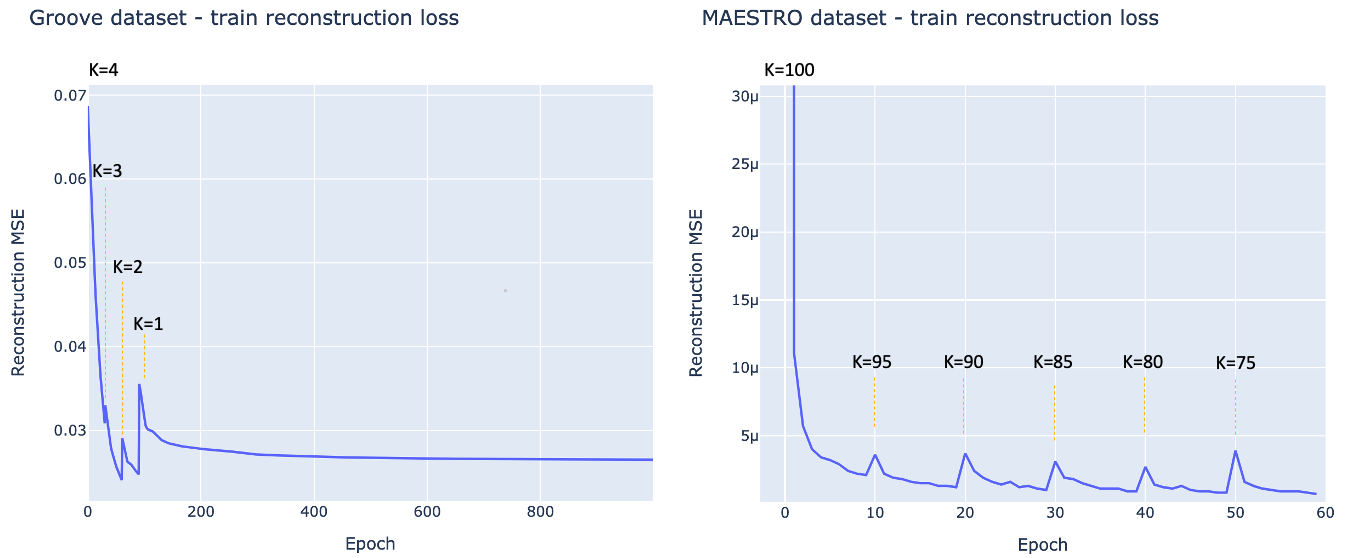
\includegraphics[width=\linewidth]{/Users/juanhuerta/personal_projects/code/shift_invariant_dictionary_learning/paper/images/maestro.png}
  \caption{After training the model we can use it to encode datapoints of arbitrary length unsupervised stylistic segmentation. We use PCA on the average sparse code for each piece. We project into 2 dimensional sparse to visualize }
  \label{fig:boat1}
\end{figure*}


\subsection{Music Reconstruction}
\label{ssec:first}

 \textbf{De-noising musical ideas: } Dictionary learning has successfully been shown to de-noise image, videos. By simply reconstructing our musical signal. 
\\
 \textbf{Keep N Active Atoms: } Another application of having a sprase code, is the ability to recognize the most used words in the dictionary. Given a sparse code we can limit a piece to only be made up of the top N atoms. Some example applications of keeping top N atoms are for example, low dimensionality feature extraction for machine learning task; music reduction--reduction wherein the complexity of the arrangement is reduced to a simpler transcription and parts. 
 %And Music Segmentation (Discretization) wherein various musical ideas used in a piece of music are isolated from the piece itself. Such segmented ideas could be used in analysis or creatively repurposed to generate new music.

\subsection{Unsupervised Stylistic Segmentation }
If we train with a dataset that includes multiple composers we should expect to find that different composers utilize different shift invariant patters. To visualize kernel usage we average out the rows of our sparse code. This should provide us with the average dictionary word value. If we do PCA on the average dictionary vector and reduce dimensionality to 2D. We obtain the plot in Figure 2

It is also possible to use this average kernel usage for each composer and make comparisons for composers, such as most similar or dissimilar between styles or comparisons. 


\subsection{Generating New Music}
 \textbf{Interpolating Sparse Code } We use encode existing music and interpolate between sparse code to generate new music. In order to obtain good results we measure cos similarity between sparse code to find candidates to interpolate. For drum generation we can all of our sections are same length; for piano we have variable length sprase code. To interpolate variable length code we can fix the input size, or interpolate specific sections of the sprase code. The results are significantly better for drum generation than piano generation. Although the piano generation does seem to follow high level musical features, such as key time, and scale.
 \\
 \textbf{Swapping atoms } Another method to generate new music, is to measure the most active atoms in the dictionary of a musical section, and replace it with the most active atom in the dictionary of a distinct section. This also can be used as a tool for artist to mix and match features of ordered importance. 


%% NOTE: NLP4MusA desn't need DOI.
% BEGIN: remove
% \textbf{Digital Object Identifiers}:  As part of our work to make ACL
% materials more widely used and cited outside of our discipline, ACL
% has registered as a CrossRef member, as a registrant of Digital Object
% Identifiers (DOIs), the standard for registering permanent URNs for
% referencing scholarly materials.  As of 2017, we are requiring all
% camera-ready references to contain the appropriate DOIs (or as a
% second resort, the hyperlinked ACL Anthology Identifier) to all cited
% works.  Thus, please ensure that you use Bib\TeX\ records that contain
% DOI or URLs for any of the ACL materials that you reference.
% Appropriate records should be found for most materials in the current
% ACL Anthology at \url{http://aclanthology.info/}.
%
% As examples, we cite \cite{P16-1001} to show you how papers with a DOI
% will appear in the bibliography.  We cite \cite{C14-1001} to show how
% papers without a DOI but with an ACL Anthology Identifier will appear
% in the bibliography.  

%  As reviewing will be double-blind, the submitted version of the papers
%  should not include the authors' names and affiliations. Furthermore,
%  self-references that reveal the author's identity, \emph{e.g.},
%  \begin{quote}
%  ``We previously showed \cite{Gusfield:97} ...''  
%  \end{quote}
%  should be avoided. Instead, use citations such as 
%  \begin{quote}
%  ``\citeauthor{Gusfield:97} \shortcite{Gusfield:97}
%  previously showed ... ''
%  \end{quote}

% Any preliminary non-archival versions of submitted papers should be listed in the submission form but not in the review version of the paper. NLP4MusA reviewers are generally aware that authors may present preliminary versions of their work in other venues, but will not be provided the list of previous presentations from the submission form. 
% END: remove




%\section{Discussion}
%\label{ssec:discussion}
%
%There are multiple benefits to this sequence learning methodology. The first is such as simplicity and felxibilty, the TCN autoencocoder is a simple to implemnt arquitecture and requires any abitrary size combinations of multivariate musical signals.Also the size of the model for both Magenta and Groove are 877 KB and 750 KB respectively. In comparison, googles Performance RNN--LSTM-based recurrent neural network--is ~25MB, and other transformer based models can be GBs in size. 
%
%In addition, our method allows for incorporating known structural information into a model prior to trainng. and finally we have the most imporant benifit is the sparse representatoin and learned dictionaries, as we have shown this can be used for mutiple applications and analysis. 
%
%The performance on the recustruction and generation on for the drum Grove dataset  was significantly better than the piano (MAESTRO dataset). This is in part because the dataset was pre-proccessed to match with kernel size, and the drum sections were the same length and have lower dimensionality. 



% Min: no longer used as of ACL 2019, following ACL exec's decision to
% remove this extra workflow that was not executed much.
% BEGIN: remove
%% \section{XML conversion and supported \LaTeX\ packages}

%% Following ACL 2014 we will also we will attempt to automatically convert 
%% your \LaTeX\ source files to publish papers in machine-readable 
%% XML with semantic markup in the ACL Anthology, in addition to the 
%% traditional PDF format.  This will allow us to create, over the next 
%% few years, a growing corpus of scientific text for our own future research, 
%% and picks up on recent initiatives on converting ACL papers from earlier 
%% years to XML. 

%% We encourage you to submit a ZIP file of your \LaTeX\ sources along
%% with the camera-ready version of your paper. We will then convert them
%% to XML automatically, using the LaTeXML tool
%% (\url{http://dlmf.nist.gov/LaTeXML}). LaTeXML has \emph{bindings} for
%% a number of \LaTeX\ packages, including the ACL 2019 stylefile. These
%% bindings allow LaTeXML to render the commands from these packages
%% correctly in XML. For best results, we encourage you to use the
%% packages that are officially supported by LaTeXML, listed at
%% \url{http://dlmf.nist.gov/LaTeXML/manual/included.bindings}
% END: remove

\section{Conclusion}

%There are multiple benefits to this sequence learning methodology. The first is such as simplicity and felxibilty, the TCN autoencocoder is a simple to implemnt arquitecture and requires any abitrary size combinations of multivariate musical signals.Also the size of the model for both Magenta and Groove are 877 KB and 750 KB respectively. In comparison, googles Performance RNN--LSTM-based recurrent neural network--is ~25MB, and other transformer based models can be GBs in size. 
%
%In addition, our method allows for incorporating known structural information into a model prior to trainng. and finally we have the most imporant benifit is the sparse representatoin and learned dictionaries, as we have shown this can be used for mutiple applications and analysis. 
%


We have shown that TCN-kWTA autoencoder can learn a sparse representation of abitrary length musical signal. This shift invariant, sparse representation can be used to analyze, preprocess, or generate musical content in a structured, or unsctuctured way

The performance on the recustruction and generation on for the drum Grove dataset  was significantly better than the piano (MAESTRO dataset). This is in part because the dataset was pre-proccessed to match with kernel size, and the drum sections were the same length and have lower dimensionality. 


\section*{Acknowledgments}

The acknowledgments should go immediately before the references.  Do
not number the acknowledgments section. Do not include this section
when submitting your paper for review. \\

\noindent \textbf{Preparing References:} \\
Include your own bib file like this:
\verb|\bibliographystyle{nlp4MusA_natbib}|
\verb|\bibliography{nlp4MusA}| 

where \verb|nlp4MusA| corresponds to a nlp4MusA.bib file.
\bibliography{SIDL-citations3}
\bibliographystyle{nlp4MusA_natbib}


\appendix

\section{Appendices}
\label{sec:appendix}
Appendices are material that can be read, and include lemmas, formulas, proofs, and tables that are not critical to the reading and understanding of the paper. 
Appendices should be \textbf{uploaded as supplementary material} when submitting the paper for review. Upon acceptance, the appendices come after the references, as shown here. Use
\verb|\appendix| before any appendix section to switch the section
numbering over to letters.


\section{Supplemental Material}
\label{sec:supplemental}
Submissions may include non-readable supplementary material used in the work and described in the paper. Any accompanying software and/or data should include licenses and documentation of research review as appropriate. Supplementary material may report preprocessing decisions, model parameters, and other details necessary for the replication of the experiments reported in the paper. Seemingly small preprocessing decisions can sometimes make a large difference in performance, so it is crucial to record such decisions to precisely characterize state-of-the-art methods. 


\end{document}
